\chapter{الكيمياء الضوئية}\label{ch:b3:photochemistry}

تبدأ الرؤية حين يثني فوتون واحد جزيئًا واحدًا. ففي الخلايا العصوية في العين،
يجلس الريتينال في بروتينه بالصورة 11-cis؛ ويحوّله فوتون من الضوء الأخضر
إلى الصورة الكلية الترانس، ويكتمل التماكب عمليًا
في غضون \qty{200}{fs}، أسرع من أي حدث كيميائي آخر تقريبًا. وبقية
عملية الرؤية، وهي تضخيم كيميائي حيوي هائل، تنتج من ذلك الجزيء
المنثني الوحيد. والقواعد نفسها (فوتون واحد يثير جزيئًا واحدًا، ثم يختار الجزيء
بين عدة مصائر) تحكم واقيات الشمس، وتخليق الحلقات المتوترة،
والعلاج الضوئي الديناميكي، والضباب الدخاني فوق المدن، \omterm{def:b3:photochemistry:chapman}{وطبقة الأوزون} التي تحمي
سطح الأرض من الأشعة فوق البنفسجية.

\begin{recall}
وصف \cref{ch:b3:electronic-spectroscopy} الحالات المثارة
للجزيئات، \omterm{def:b3:electronic-spectroscopy:jablonski}{ومخطط يابلونسكي}، \omterm{def:b3:electronic-spectroscopy:radiationless}{والعبور بين الأنظمة}، \omterm{def:b3:electronic-spectroscopy:luminescence}{والتفلور} 
\omterm{def:b3:electronic-spectroscopy:luminescence}{والتفسفر}، والإخماد \omterm{def:b3:electronic-spectroscopy:quantum-yield}{والمردود الكمي} لعملية فيزيائية ضوئية.
وعرّف مجلد السنة الأولى الجذور الحرة، والانشطار المتجانس والمتماكبات $Z$/$E$؛ وعرّف مجلد السنة الثانية
التفاعلات المتضافرة والمدارات الحدودية والدورات الحفزية.
وعالج \cref{ch:b3:complex-kinetics} \omterm{def:b3:complex-kinetics:chain}{التفاعلات المتسلسلة} والحالات المستقرة.
\end{recall}

\section{الضوء كاشفًا}

مبدآن قديمان يفتتحان الموضوع: لا يستطيع أن يُحدث تغيرًا كيميائيًا إلا الضوء
الممتص (غروتوس ودرابر)، وكل فوتون ممتص يثير جزيئًا
واحدًا (شتارك وأينشتاين).

\begin{definition}[تدفق الفوتونات، المقياس الأكتيني الكيميائي]\label{def:b3:photochemistry:photon-flux}
\emph{تدفق الفوتونات}\index{تدفق الفوتونات} من مصدر ضوئي هو عدد
الفوتونات التي يقدّمها في وحدة الزمن، ويُعدّ غالبًا بمولات الفوتونات (الأينشتاين)
في الثانية. و\emph{المقياس الأكتيني الكيميائي}\index{مقياس أكتيني كيميائي}
تفاعل كيميائي ضوئي معروف \omterm{def:b3:electronic-spectroscopy:quantum-yield}{المردود الكمي} بدقة يُستعمل لقياس
تدفق الفوتونات.
\end{definition}

\begin{proposition}[قانون شتارك--أينشتاين]\label{prop:b3:photochemistry:stark-einstein}
في شدات الضوء العادية، يثير كل فوتون ممتص جزيئًا واحدًا
بالضبط؛ ومجموع المردودات الكمية الأولية لكل العمليات التي تنطلق من
الحالة المثارة يساوي 1.
\end{proposition}

\begin{proof}[برهان جزئي]
نقبل دون برهان أن الفوتون الواحد يمتصه جزيء واحد في كل مرة (فامتصاص
فوتونين يحتاج إلى شدات الليزرات النبضية). ثم يختفي الجزيء المثار
بعمليات متنافسة من الرتبة الأولى ثوابت سرعتها $k_i$
(\cref{ch:b3:electronic-spectroscopy}): فالنسبة التي تسلك الطريق $i$ هي $\Phi_i =
k_i/\sum_jk_j$، و$\sum_i\Phi_i = 1$.
\end{proof}

\omterm{def:b3:electronic-spectroscopy:quantum-yield}{المردود الكمي} لتفاعل، أي عدد الجزيئات المحوَّلة لكل فوتون
ممتص، لا يخضع بالضرورة لهذا الحد: فالخطوة الكيميائية الضوئية الأولية قد تبدأ
سلسلة. فخليط من \ce{H2} و\ce{Cl2} معرَّض للضوء يتفاعل بمردودات كمية
تبلغ $10^4$ وأكثر، إذ يبدأ كل جزيء \ce{Cl2} متحلل ضوئيًا سلسلة مثل سلسلة
تفاعل الهيدروجين--البروم في \cref{ch:b3:complex-kinetics}؛ \omterm{def:b3:electronic-spectroscopy:quantum-yield}{فالمردود الكمي}
الأكبر من 1 علامة على وجود سلسلة.

\begin{proposition}[سرعة تفاعل كيميائي ضوئي]\label{prop:b3:photochemistry:rate}
المحلول ذو الامتصاصية $A$ عند طول موجة التشعيع، الذي يتلقى تدفق فوتونات
$I_0$ (أينشتاين في الثانية)، يمتص $I_{\mathrm{abs}} = I_0(1 - 10^{-A})$؛ وإذا
امتص المتفاعل كل ذلك، حوّل التفاعل $v = \Phi I_{\mathrm{abs}}$ مولًا في الثانية.
\end{proposition}

\begin{proof}
بحسب قانون بير--لامبرت يكون التدفق النافذ $I_010^{-A}$، فالتدفق الممتص
$I_0(1 - 10^{-A})$؛ وبحسب تعريف \omterm{def:b3:electronic-spectroscopy:quantum-yield}{المردود الكمي}، يتفاعل $\Phi$ جزيئًا لكل
فوتون ممتص.
\end{proof}

\begin{method}[سرعة تفاعل ضوئي انطلاقًا من المصباح]\label{met:b3:photochemistry:photochemical-rate}
\begin{enumerate}
  \item طاقة الفوتون $E = hc/\lambda$؛ \omterm{def:b3:photochemistry:photon-flux}{وتدفق الفوتونات} $I_0 = P/E$ لاستطاعة $P$ تبلغ
        العيّنة، أو يُقاس بمقياس أكتيني؛ واقسم على $N_A$ للحصول على الأينشتاين في
        الثانية.
  \item النسبة الممتصة $1 - 10^{-A}$، مع $A$ عند طول موجة التشعيع (وهي
        تتغير مع استهلاك المتفاعل).
  \item السرعة $\Phi I_{\mathrm{abs}}$ بوحدة mol/s، مقسومة على الحجم للحصول على سرعة بالتركيز.
\end{enumerate}
\end{method}

\begin{method}[القياس الأكتيني بالفيريأوكسالات]\label{met:b3:photochemistry:actinometry}
\begin{enumerate}
  \item شعّع، في الخلية نفسها وبالهندسة نفسها اللتين في التجربة، محلولًا محمَّضًا
        من ثلاثي(أوكسالاتو)فيرات(III) البوتاسيوم، مركّزًا بما يكفي
        ليمتص عمليًا كل الضوء دون نحو \qty{450}{nm}.
  \item يختزل الضوء Fe(III) إلى Fe(II) \omterm{def:b3:electronic-spectroscopy:quantum-yield}{بمردود كمي} معايَر؛ وبعد
        زمن مقيس، أضف 1،10-فينانترولين ومحلولًا منظِّمًا، وقِس
        امتصاصية المعقد الأحمر $\ce{[Fe(phen)3]^{2+}}$.
  \item مولات Fe(II) مقسومة على (\omterm{def:b3:electronic-spectroscopy:quantum-yield}{المردود الكمي} $\times$ الزمن) تعطي \omterm{def:b3:photochemistry:photon-flux}{تدفق الفوتونات}.
\end{enumerate}
\end{method}

\section{التفاعلات الكيميائية الضوئية}

\begin{definition}[التماكب الضوئي، الحالة المستقرة ضوئيًا]\label{def:b3:photochemistry:photoisomerisation}
\emph{التماكب الضوئي}\index{تماكب ضوئي} تحويل يُحدثه الضوء
لمتماكب إلى آخر، عادة $E \to Z$ حول رابطة مضاعفة. وتحت
تشعيع مستمر يبلغ متماكبان يمتص كلاهما
\emph{حالة مستقرة ضوئيًا}\index{حالة مستقرة ضوئيًا}، أي تركيبًا ثابتًا
يحدده الضوء، لا الترموديناميك.
\end{definition}

يفسّر التواء الرابطة المضاعفة لماذا يُحدث الضوء تماكب الألكينات. ففي
الحالة الأساسية ترتفع الطاقة كلما التوى الطرفان، إلى قيمة عظمى عند $90^\circ$
حيث تنكسر الرابطة $\pi$. أما في الحالة المثارة $\pi\pi^*$ فينقلب الترتيب:
فالهندسة الملتوية هي الأكثر استقرارًا. فيلتوي الجزيء المثار نحو
$90^\circ$، حيث يتقارب السطحان، ويعود هناك إلى الحالة الأساسية،
ويسقط إلى أحد الجانبين: إلى المتماكب الذي انطلق منه أو إلى
الآخر.

\begin{omfigure}
\begin{tikzpicture}[font=\small, >=Stealth, x=0.032cm, y=1.1cm]
  \draw[->] (0,0) -- (195,0);
  \node[anchor=north] at (135,-0.45) {\foreignlanguage{arabic}{زاوية الالتواء}};
  \draw[->] (0,0) -- (0,5.2) node[anchor=south] {\foreignlanguage{arabic}{الطاقة}};
  \foreach \t/\l in {0/{0^\circ}, 90/{90^\circ}, 180/{180^\circ}}{
    \draw (\t,0) -- (\t,-0.08) node[anchor=north] {$\l$};}
  \draw[thick, black, domain=0:180, samples=90] plot (\x,{2.6*sin(\x)^2 + 0.15*(1-cos(\x))/2});
  \draw[thick, omThm, domain=0:180, samples=90] plot (\x,{4.5 - 1.6*sin(\x)^2 + 0.1*(1-cos(\x))/2});
  \node[anchor=east] at (0,0.15) {$E$};
  \node[anchor=west] at (182,0.2) {$Z$};
  \node[omThm, anchor=south west] at (5,4.55) {$\mathrm S_1$ ($\pi\pi^*$)};
  \node[anchor=north west] at (52,1.2) {$\mathrm S_0$};
  \draw[->, omDef, thick] (12,0.12) -- (12,4.4) node[midway, left] {$h\nu$};
  \draw[->, omDef, thick, decorate, decoration={snake, amplitude=0.6mm, segment length=3mm}] (16,4.4) -- (80,3.05);
  \draw[->, omDef, thick] (90,2.85) -- (90,2.75);
  \draw[->, black!60, thick, domain=96:168, samples=40] plot (\x,{2.6*sin(\x)^2 + 0.15*(1-cos(\x))/2 + 0.28});
  \draw[->, black!60, thick, domain=84:12, samples=40] plot (\x,{2.6*sin(\x)^2 + 0.15*(1-cos(\x))/2 + 0.28});
  \node[font=\scriptsize, anchor=south, align=center] at (90,3.05) {\foreignlanguage{arabic}{القُمع}};
\end{tikzpicture}

{\small الحالة الأساسية ($\mathrm S_0$) والحالة المثارة الأولى ($\mathrm S_1$) لألكين بدلالة
التواء رابطته المضاعفة (رسم تخطيطي). تعقب إثارةَ المتماكب $E$ (السهم العمودي)
التواءٌ على $\mathrm S_1$ حتى الهندسة المتعامدة، حيث يكاد
السطحان يتلامسان؛ فيعود الجزيء إلى $\mathrm S_0$ هناك ويسترخي إلى $E$ أو إلى
$Z$.}
\end{omfigure}

\begin{proposition}[التركيب المستقر ضوئيًا]\label{prop:b3:photochemistry:pss}
تحت تشعيع أحادي اللون لمحلول رقيق ضوئيًا، يبلغ متماكبان $E$
و$Z$ معاملا امتصاصهما $\varepsilon_E$ و$\varepsilon_Z$ ومردوداهما الكميان $\Phi_{E\to Z}$
و$\Phi_{Z\to E}$ النسبة المستقرة ضوئيًا
\[
  \frac{[Z]}{[E]} = \frac{\varepsilon_E\Phi_{E\to Z}}{\varepsilon_Z\Phi_{Z\to E}} .
\]
\end{proposition}

\begin{proof}
في عيّنة رقيقة ضوئيًا يمتص كل متماكب تدفقًا متناسبًا مع $\varepsilon[\cdot]$، ومنه
$\dd[Z]/\dd t = c(\varepsilon_E\Phi_{E\to Z}[E] - \varepsilon_Z\Phi_{Z\to E}[Z])$ حيث $c$ ثابت يحدده الضوء؛
والحالة المستقرة تجعل ما بين القوسين معدومًا. (وتصح النتيجة أيضًا للعيّنات
السميكة، إذ يتقاسم المتماكبان عندئذ الضوء الممتص بالنسبة نفسها.)
\end{proof}

\begin{omfigure}
\begin{tikzpicture}
\begin{axis}[width=0.7\linewidth, height=5.0cm, xmin=0, xmax=120, ymin=0, ymax=1,
  axis lines=left, xlabel={\foreignlanguage{arabic}{زمن التشعيع \babelsublr{(s)}}}, ylabel={\foreignlanguage{arabic}{نسبة $Z$}},
  tick label style={font=\small}, label style={font=\small}]
\addplot[omDef, very thick] table[x=t, y=Z] {figdata/out/bachelor-3-photostationary.dat};
\draw[black!35, densely dotted] (axis cs:0,0.801) -- (axis cs:60,0.801);
\draw[black!35, densely dotted] (axis cs:60,0.161) -- (axis cs:120,0.161);
\draw[black!35] (axis cs:60,0) -- (axis cs:60,1);
\node[font=\scriptsize, anchor=north] at (axis cs:30,0.98) {\qty{365}{nm}};
\node[font=\scriptsize, anchor=north] at (axis cs:90,0.98) {\qty{440}{nm}};
\node[font=\scriptsize, anchor=south east] at (axis cs:58,0.81) {\shortstack{\foreignlanguage{arabic}{مستقرة ضوئيًا}\\ 0.80}};
\node[font=\scriptsize, anchor=south east] at (axis cs:118,0.17) {\foreignlanguage{arabic}{مستقرة ضوئيًا \babelsublr{0.16}}};
\end{axis}
\end{tikzpicture}

{\small مبدّل ضوئي نموذجي (جزيء شبيه بالأزوبنزين) يُشعَّع عند \qty{365}{nm}، حيث
يمتص المتماكب $E$ أقوى بكثير، ثم عند \qty{440}{nm}، حيث يمتص المتماكب $Z$ أقوى:
فيتنقل التركيب بين حالتين مستقرتين ضوئيًا (معاملات امتصاص
ومردودات كمية نموذجية).}
\end{omfigure}

تماكب الريتينال من الصورة 11-cis إلى الصورة الكلية الترانس في الرودوبسين تفاعل من هذا النوع،
يجعله البروتين سريعًا وانتقائيًا على نحو استثنائي. وتُستعمل المبدّلات الضوئية
الاصطناعية المبنية على الأزوبنزين أو الستيلبين للتحكم بالضوء في الآلات
الجزيئية والمواد، وفي النشاط الحيوي حين تُربط بأدوية أو بقنوات
أيونية.

\begin{definition}[التحلل الضوئي]\label{def:b3:photochemistry:photolysis}
\emph{التحلل الضوئي}\index{تحلل ضوئي} كسر رابطة بالضوء. وفي
الغلاف الجوي، ثابت السرعة من الرتبة الأولى $j$ للتحلل الضوئي لنوع ما، أي
\emph{ثابت سرعة التحلل الضوئي}\index{ثابت سرعة التحلل الضوئي} له، هو مجموعٌ على
أطوال الموجات لجداء \omterm{def:b3:photochemistry:photon-flux}{تدفق الفوتونات} الشمسي في المقطع العرضي للامتصاص في
\omterm{def:b3:electronic-spectroscopy:quantum-yield}{المردود الكمي}.
\end{definition}

لا يكسر الفوتون رابطة إلا إذا تجاوزت طاقته طاقة التفكك:
$\lambda < hcN_A/D_0$. ومن أجل \ce{O2}، $D_0 = 2\Delta_fH^\circ_0(\ce{O}) = \qty{493.6}{kJ/mol}$ من الجداول
الترموكيميائية، فلا يستطيع شطره إلا الضوء الأقصر من \qty{242}{nm}.

تكوّن الكيتونات والألكينات المثارة روابط أيضًا. فألكينان، أحدهما مثار،
يتحدان في سيكلوبيوتان: وهي الإضافة الحلقية الضوئية $[2+2]$، الممنوعة في
الحالة الأساسية والمسموحة في الحالة المثارة لأسباب مدارية تُعطى في
\cref{ch:b3:pericyclic}. وهي تصنع حلقات رباعية، متوترة ويصعب
بلوغها بغير ذلك، في خطوة واحدة.

\begin{definition}[تفاعلات نوريش]\label{def:b3:photochemistry:norrish}
\emph{تفاعل نوريش من النوع الأول}\index{تفاعل نوريش من النوع الأول} هو انشطار الرابطة بين
كربون الكربونيل وكربون $\alpha$ في كيتون مثار،
إلى جذر أسيل وجذر ألكيل. و\emph{تفاعل نوريش من النوع
الثاني}\index{تفاعل نوريش من النوع الثاني} هو انتزاع أكسجين
كيتون مثار ذرة هيدروجين من الكربون $\gamma$، فيعطي ثنائي جذر 1،4
ينشطر إلى إينول وألكين أو ينغلق في سيكلوبيوتانول.
\end{definition}

\begin{omfigure}
\setchemfig{atom sep=1.9em}
\schemestart
\chemfig{H_3C-[:30]C(=[:90]O)-[:-30]CH_2-[:30]CH_2-[:-30]CH_2-[:30]CH_3}
\arrow{->[$h\nu$][عبر $\mathrm T_1$]}
\chemfig{H_3C-[:30]\chembelow{C}{\scriptstyle\bullet}(-[:90]OH)-[:-30]CH_2-[:30]CH_2-[:-30]\chemabove{C}{\scriptstyle\bullet}H-[:30]CH_3}
\schemestop

\medskip
\schemestart
\arrow{->[انشطار]}[,1.1]
\chemfig{H_3C-[:30]C(-[:90]OH)=[:-30]CH_2}
\+
\chemfig{H_2C=[:30]CH-[:-30]CH_3}
\schemestop
\hspace{2.5em}
\schemestart
\arrow{->[إغلاق][الحلقة]}[,1.1]
\chemfig{*4(-(-[::-40]OH)(-[::40]CH_3)-(-CH_3)---)}
\schemestop
\par\medskip

{\small \omterm{def:b3:photochemistry:norrish}{تفاعل نوريش من النوع الثاني} للهكسان-2-ون. ينتزع الكيتون الثلاثي
ذرة هيدروجين من الكربون $\gamma$ عبر ترتيب سداسي الحلقة؛ وثنائي الجذر 1،4
ينشطر إلى إينول الأسيتون (الذي يتصاوغ إلى أسيتون) والبروبين،
أو ينغلق في 1،2-ثنائي ميثيل سيكلوبيوتان-1-ول.}
\end{omfigure}

الاختزال الضوئي للبنزوفينون هو الصورة الثنائية الجزيئية الكلاسيكية: فحالته
الثلاثية تنتزع ذرة هيدروجين من مذيب كحولي مثل البروبان-2-ول،
وتقترن جذور ثنائي فينيل هيدروكسي ميثيل الناتجة مثنى مثنى في البنزوبيناكول،
الذي يتبلور من المحلول.

\section{التحسيس الضوئي}

\begin{definition}[التحسيس الضوئي، الأكسجين الأحادي]\label{def:b3:photochemistry:sensitisation}
\emph{المحسِّس الضوئي}\index{محسِّس ضوئي} جزيء يمتص الضوء
وينقل الطاقة أو إلكترونًا إلى جزيء آخر لا
يمتص بنفسه: وهذا هو \emph{التحسيس الضوئي}\index{تحسيس ضوئي}. وفي
\emph{نقل الطاقة الثلاثية}\index{نقل الطاقة الثلاثية} تعطي \omterm{def:b3:many-electron-atoms:singlet-triplet}{الحالة الثلاثية}
للمحسِّس، المتكوّنة \omterm{def:b3:electronic-spectroscopy:radiationless}{بالعبور بين الأنظمة}، طاقتها للمستقبِل
عند التماس، فتترك المستقبِل في حالته الثلاثية. و\emph{الأكسجين
الأحادي}\index{أكسجين أحادي} أدنى حالة مثارة للجزيء \ce{O2}،
${}^1\Delta_g$، تتكوّن على هذا النحو من الأكسجين في حالته الأساسية ${}^3\Sigma_g^-$.
\end{definition}

\begin{proposition}[شرط الطاقة في النقل الثلاثي]\label{prop:b3:photochemistry:sensitisation-condition}
يقترب نقل الطاقة ثلاثي--ثلاثي من مانح D إلى مستقبل A من
حد الانتشار حين تتجاوز $E_{\mathrm T}(\mathrm D)$ قيمة $E_{\mathrm T}(\mathrm A)$ بأكثر من نحو \qty{10}{kJ/mol}، 
وينخفض بشدة حين يصير الفرق سالبًا.
\end{proposition}

\begin{proof}[برهان جزئي]
النقل ${}^3\mathrm D + \mathrm A \to \mathrm D + {}^3\mathrm A$ يحفظ السبين (حالتان ثلاثية وأحادية تحلان محل
أحادية وثلاثية) ويحتاج إلى تماس مداري (آلية تبادل،
نقبلها دون برهان). وثابت توازنه $\exp[(E_{\mathrm T}(\mathrm D) - E_{\mathrm T}(\mathrm A))/RT]$، نحو 60 من أجل
فائض قدره \qty{10}{kJ/mol} عند \qty{298}{K}: فتحدث الخطوة الأمامية عندئذ عند كل
لقاء تقريبًا. وحين يكون الفرق سالبًا، يكون ثابت السرعة الأمامي هو
حد الانتشار مضروبًا في مقلوب ذلك العامل (فالاتجاه الصاعد يدفع
عامل بولتزمان)؛ ونقبل المنحنى الكمي دون برهان.
\end{proof}

المحسِّس الجيد يمتص حيث لا يمتص المستقبِل، ويعبر إلى حالته الثلاثية
بمردود عالٍ، ولحالته الثلاثية عمر طويل: والبنزوفينون، الذي يقارب
مردوده الثلاثي 1، هو المرجع. \omterm{def:b3:photochemistry:sensitisation}{والأكسجين الأحادي} محب للإلكترونات
تفاعلي: يُضاف إلى الديينات وإلى الألكينات الغنية بالإلكترونات. وفي العلاج
الضوئي الديناميكي، يكوّن محسِّسٌ يتراكم في ورم، ويُضاء عبر
ليف بصري، أكسجينًا أحاديًا يدمّر الخلايا المحيطة به.

\begin{definition}[الحفز الضوئي بالأكسدة والاختزال]\label{def:b3:photochemistry:photoredox}
يستعمل \emph{الحفز الضوئي بالأكسدة والاختزال}\index{حفز ضوئي بالأكسدة والاختزال} محسِّسًا ضوئيًا
تكون حالته المثارة مؤكسدًا أقوى ومختزلًا أقوى معًا من
حالته الأساسية، لنقل إلكترونات مفردة إلى الركائز أو منها، فيولّد
جذورًا حرة تحت الضوء المرئي؛ ويُجدَّد المحسِّس في دورة
حفزية.
\end{definition}

المعقد الروثينيومي $\ce{[Ru(bpy)3]^{2+}}$ هو النموذج الأولي: فحالته المثارة لنقل الشحنة من الفلز إلى
الربيطة، التي تُبلغ بالضوء الأزرق وتعيش نحو
ميكروثانية، تستطيع أن تأخذ إلكترونًا من أمين أو أن تعطي إلكترونًا لهاليد
عضوي. وتشارك الجذور المتكوّنة في تفاعلات تكوّن روابط في
ظروف أكثر اعتدالًا بكثير من ظروف كيمياء الجذور الكلاسيكية.

\section{الكيمياء الضوئية للغلاف الجوي}

\begin{definition}[آلية تشابمان، طبقة الأوزون]\label{def:b3:photochemistry:chapman}
\emph{آلية تشابمان}\index{آلية تشابمان} هي مجموعة الخطوات الأربع
\[
  \ce{O2 ->[h\nu] 2 O}\ (j_1), \quad \mathrm{O + O_2 + M \to O_3 + M}\ (k_2), \quad
  \ce{O3 ->[h\nu] O2 + O}\ (j_3), \quad \ce{O + O3 -> 2 O2}\ (k_4).
\]
و\emph{طبقة الأوزون}\index{طبقة الأوزون} هي منطقة الستراتوسفير، على ارتفاع
نحو 15 إلى \qty{35}{km} فوق الأرض، حيث تحافظ هذه التفاعلات على أعلى
تراكيز الأوزون.
\end{definition}

\begin{theorem}[الحالة المستقرة لتشابمان]\label{thm:b3:photochemistry:chapman}
في \omterm{def:b3:photochemistry:chapman}{آلية تشابمان}، يبلغ O و\ce{O3} الحالة المستقرة
\[
  \frac{[\ce{O}]}{[\ce{O3}]} = \frac{j_3}{k_2[\mathrm M][\ce{O2}]}, \qquad
  [\ce{O3}] = [\ce{O2}]\sqrt{\frac{j_1k_2[\mathrm M]}{j_3k_4}} .
\]
\end{theorem}

\begin{proof}
يتحول O و\ce{O3} أحدهما إلى الآخر بسرعة عبر الخطوتين 2 و3 (ثوانٍ)، أسرع بكثير
مما يتكوّنان أو يُتلفان: وبجعل التبادل السريع في توازن،
$k_2[\ce{O}][\ce{O2}][\mathrm M] = j_3[\ce{O3}]$، نحصل على النسبة. ومجموعهما، الأكسجين الفردي، تكوّنه
الخطوة 1 (ذرتا O لكل \ce{O2}) وتُتلفه الخطوة 4 (أكسجينان فرديان في كل حدث):
$2j_1[\ce{O2}] = 2k_4[\ce{O}][\ce{O3}]$. وتعويض $[\ce{O}]$ من النسبة يعطي $[\ce{O3}]^2 = j_1k_2[\mathrm M][\ce{O2}]^2/(j_3k_4)$.
\end{proof}

بثوابت السرعة المأخوذة من قاعدة المعطيات المقيَّمة وسرعات \omterm{def:b3:photochemistry:photolysis}{تحلل ضوئي} نموذجية
لارتفاع \qty{30}{km} (معطيات مسألة نهاية الأسبوع)، يعطي نموذج تشابمان نحو
$\num{6e12}$ جزيء أوزون في كل \unit{cm^3}، أي نحو خمسة عشر جزءًا من المليون. وبالمكاملة على
الارتفاع، يحتوي الغلاف الجوي كله في المتوسط على نحو 300 وحدة دوبسون من الأوزون:
أي طبقة سمكها \qty{3}{mm} إذا ضُغطت إلى ضغط السطح. \omterm{def:b3:photochemistry:chapman}{وآلية تشابمان}
وحدها تتنبأ بأكثر مما يُرصد: فالدورات الحفزية تُتلف الأوزون أسرع.

\begin{definition}[استنفاد الأوزون، الأنواع الخازنة]\label{def:b3:photochemistry:ozone-depletion}
\emph{استنفاد الأوزون}\index{استنفاد الأوزون} هو تناقص عمود
الأوزون الستراتوسفيري بفعل دورات حفزية من الجذور الحرة (Cl وClO،
وNO و\ce{NO2}، وOH و\ce{HO2}). و\emph{النوع الخازن}\index{نوع خازن}
جزيء مستقر (HCl، \ce{ClONO2}) يحتفظ بجذر حفزي في صورة غير نشطة،
يمكن أن يتحرر منها لاحقًا.
\end{definition}

\begin{omfigure}
\begin{tikzpicture}[font=\small, >=Stealth]
  \node (cl) at (0,0) {Cl};
  \node (clo) at (3.2,0) {ClO};
  \draw[->, thick, omThm] (cl) to[bend left=40] node[midway, above] {$+\,\ce{O3}$, $-\,\ce{O2}$} (clo);
  \draw[->, thick, omThm] (clo) to[bend left=40] node[midway, below] {$+\,\ce{O}$, $-\,\ce{O2}$} (cl);
  \node[font=\scriptsize, align=center] at (1.6,0) {\foreignlanguage{arabic}{المحصلة}\\ $\ce{O + O3 -> 2 O2}$};
  \draw[->, black!55] (cl) -- (-1.6,-1.2) node[below, font=\scriptsize] {$+\,\ce{CH4} \to$ HCl};
  \draw[->, black!55] (clo) -- (4.8,-1.2) node[below, font=\scriptsize] {$+\,\ce{NO2} \to \ce{ClONO2}$};
  \node (o2) at (8.0,1.3) {\ce{O2}};
  \node (o) at (8.0,-1.1) {O};
  \node (o3) at (11.4,-1.1) {\ce{O3}};
  \draw[->, thick] (o2) -- (o) node[midway, left, font=\scriptsize] {$h\nu$};
  \draw[->, thick] (o.south east) to[bend right=30] node[midway, below, font=\scriptsize] {$+\,\ce{O2}$, M} (o3.south west);
  \draw[->, thick] (o3.north west) to[bend right=30] node[midway, above, font=\scriptsize] {$h\nu$} (o.north east);
  \draw[->, thick, black!55] (o3.north) -- (o2.east) node[midway, above right, font=\scriptsize] {$+\,\ce{O}$};
\end{tikzpicture}

{\small يسارًا: الدورة الحفزية للكلور، التي تُتلف جزيء أوزون واحدًا 
وذرة أكسجين واحدة في كل دورة وتعيد ذرة الكلور؛ والأسهم الرمادية تقود
إلى الخزانات. يمينًا: دورة تشابمان، التي يتبادل فيها \ce{O} و\ce{O3}
بسرعة بالاتحاد \omterm{def:b3:photochemistry:photolysis}{والتحلل الضوئي} بينما تكوّن الخطوات البطيئة الأكسجين الفردي وتُتلفه.}
\end{omfigure}

\begin{proposition}[طول سلسلة دورة الكلور]\label{prop:b3:photochemistry:catalytic-destruction}
إذا تفاعلت ذرة Cl في كل دورة مع \ce{O3} باحتمال $p_1 =
k[\ce{O3}]/(k[\ce{O3}] + k'[\ce{CH4}])$ وتفاعل الجذر ClO مع O باحتمال $p_2 =
k''[\ce{O}]/(k''[\ce{O}] + k'''[\ce{NO2}])$، فإن متوسط عدد الدورات قبل أن يُحتجز الكلور
في خزان هو $p/(1 - p)$ مع $p = p_1p_2$؛ وكل دورة تُتلف جزيء
أوزون واحدًا.
\end{proposition}

\begin{proof}
تكتمل كل دورة باحتمال $p$، باستقلال عن الدورات
السابقة: فعدد الدورات المكتملة $n$ قبل الاحتجاز احتماله $p^n(1 -
p)$، و$\sum_nnp^n(1 - p) = p/(1 - p)$.
\end{proof}

\begin{omfigure}
\begin{tikzpicture}
\begin{axis}[name=oc, width=0.47\linewidth, height=5.2cm, xmin=0, xmax=120, ymin=0, ymax=6.4,
  axis lines=left, xlabel={\foreignlanguage{arabic}{الزمن بالأيام}}, ylabel={\babelsublr{$[\ce{O3}]$ / $10^{12}$ \unit{cm^{-3}}}},
  tick label style={font=\small}, label style={font=\small},
  legend style={font=\scriptsize, draw=none, fill=white, fill opacity=0.85, text opacity=1,
  at={(0.97,0.03)}, anchor=south east}, legend cell align=left, title={\small \foreignlanguage{arabic}{الستراتوسفير}}]
\addplot[black, thick] table[x=day, y=noCl] {figdata/out/bachelor-3-ozone-chemistry-chapman.dat};
\addplot[omDef, thick] table[x=day, y=Cl1] {figdata/out/bachelor-3-ozone-chemistry-chapman.dat};
\addplot[omThm, thick] table[x=day, y=Cl3] {figdata/out/bachelor-3-ozone-chemistry-chapman.dat};
\legend{{\foreignlanguage{arabic}{تشابمان}}, {\babelsublr{$+$ \qty{1e7}{cm^{-3}} ClO$_x$}}, {\babelsublr{$+$ \qty{3e7}{cm^{-3}} ClO$_x$}}}
\end{axis}
\begin{axis}[at={(oc.east)}, anchor=west, xshift=1.5cm, width=0.47\linewidth, height=5.2cm,
  xmin=0, xmax=4, ymin=0, ymax=80, axis lines=left, xlabel={$[\ce{NO2}]/[\ce{NO}]$},
  ylabel={\foreignlanguage{arabic}{$[\ce{O3}]$ بأجزاء من المليار}}, tick label style={font=\small}, label style={font=\small},
  title={\small \foreignlanguage{arabic}{هواء ملوث عند الظهيرة}}]
\addplot[omDef, very thick] table[x=ratio, y=O3ppb] {figdata/out/bachelor-3-ozone-chemistry-leighton.dat};
\end{axis}
\end{tikzpicture}

{\small يسارًا: الأوزون عند ارتفاع نموذجي نحو \qty{30}{km} (\qty{230}{K}، وثوابت سرعة
مقيَّمة، وسرعات \omterm{def:b3:photochemistry:photolysis}{التحلل الضوئي} في مسألة نهاية الأسبوع)، يتراكم انطلاقًا من الصفر
وفق \omterm{def:b3:photochemistry:chapman}{آلية تشابمان}، ويكون أدنى بوجود دورة الكلور. يمينًا: \omterm{def:b3:photochemistry:photoisomerisation}{الحالة
المستقرة ضوئيًا} لليتون في هواء ملوث عند \qty{298}{K}، $[\ce{O3}] = j[\ce{NO2}]/k[\ce{NO}]$ مع
$j = \qty{8e-3}{s^{-1}}$ (قيمة نموذجية عند الظهيرة).}
\end{omfigure}

كل ذرة كلور، تتحرر في الستراتوسفير من مركبات الكلوروفلوروكربون
\omterm{def:b3:photochemistry:photolysis}{بالتحلل الضوئي} فوق البنفسجي، تُتلف الأوزون في عشرات الدورات قبل أن تُخزَّن في صورة
HCl أو \ce{ClONO2}، ثم تتحرر من جديد مرات كثيرة خلال السنوات التي تقضيها
هناك. وفوق القارة القطبية الجنوبية، في الليل القطبي، تتكوّن سحب من الجليد ومن
هيدرات حمض النتريك؛ وعلى سطوحها يتفاعل الخزانان معًا،
$\ce{HCl + ClONO2 -> Cl2 + HNO3}$، ويبقى حمض النتريك في الجسيمات، وحين
تعود الشمس في الربيع يتحلل \ce{Cl2} ضوئيًا: ومع إزالة \ce{NO2}، لا يُحتجز الكلور
من جديد، وتُتلف دورةٌ عبر ثنائي ClO الأوزونَ دون
حاجة إلى ذرات O. فينخفض عمود الأوزون إلى نحو 100 وحدة دوبسون: وهذا ثقب
الأوزون.

\begin{proposition}[علاقة ليتون]\label{prop:b3:photochemistry:leighton}
في هواء مُشمس لا يتكوّن فيه الأوزون إلا \omterm{def:b3:photochemistry:photolysis}{بالتحلل الضوئي} للمركب \ce{NO2} ولا يُتلف
إلا بالمركب NO، تبلغ الأنواع الثلاثة \omterm{def:b3:photochemistry:photoisomerisation}{الحالة المستقرة ضوئيًا}
\[
  [\ce{O3}] = \frac{j_{\ce{NO2}}[\ce{NO2}]}{k[\ce{NO}]} .
\]
\end{proposition}

\begin{proof}
$\ce{NO2 ->[h\nu] NO + O}$ ($j_{\ce{NO2}}$)، $\mathrm{O + O_2 + M \to O_3 + M}$ (سريعة: كل ذرة O تكوّن جزيء \ce{O3})، 
و$\ce{NO + O3 -> NO2 + O2}$ ($k$): في الحالة المستقرة يساوي الأوزون المتكوّن، $j_{\ce{NO2}}[\ce{NO2}]$،
الأوزون المُتلَف، $k[\ce{NO}][\ce{O3}]$.
\end{proof}

لا تكوّن الدورة وحدها أي أوزون صافٍ: فهي لا تفعل إلا تبادل NO و\ce{NO2} و\ce{O3}. وما
يرفع النسبة $[\ce{NO2}]/[\ce{NO}]$، ومنه الأوزون، هو أكسدة NO إلى \ce{NO2}
دون استهلاك الأوزون، بجذور البيروكسي الآتية من أكسدة
الهيدروكربونات بالجذر OH، منظّف التروبوسفير.

\begin{definition}[الضباب الدخاني الكيميائي الضوئي]\label{def:b3:photochemistry:smog}
\emph{الضباب الدخاني الكيميائي الضوئي}\index{ضباب دخاني كيميائي ضوئي} خليط من الأوزون 
وثنائي أكسيد النيتروجين والألدهيدات ونترات البيروكسي أسيل والجسيمات الدقيقة المتكوّن في
هواء مُشمس ملوث بأكاسيد النيتروجين والمركبات العضوية المتطايرة.
\end{definition}

\begin{omfigure}
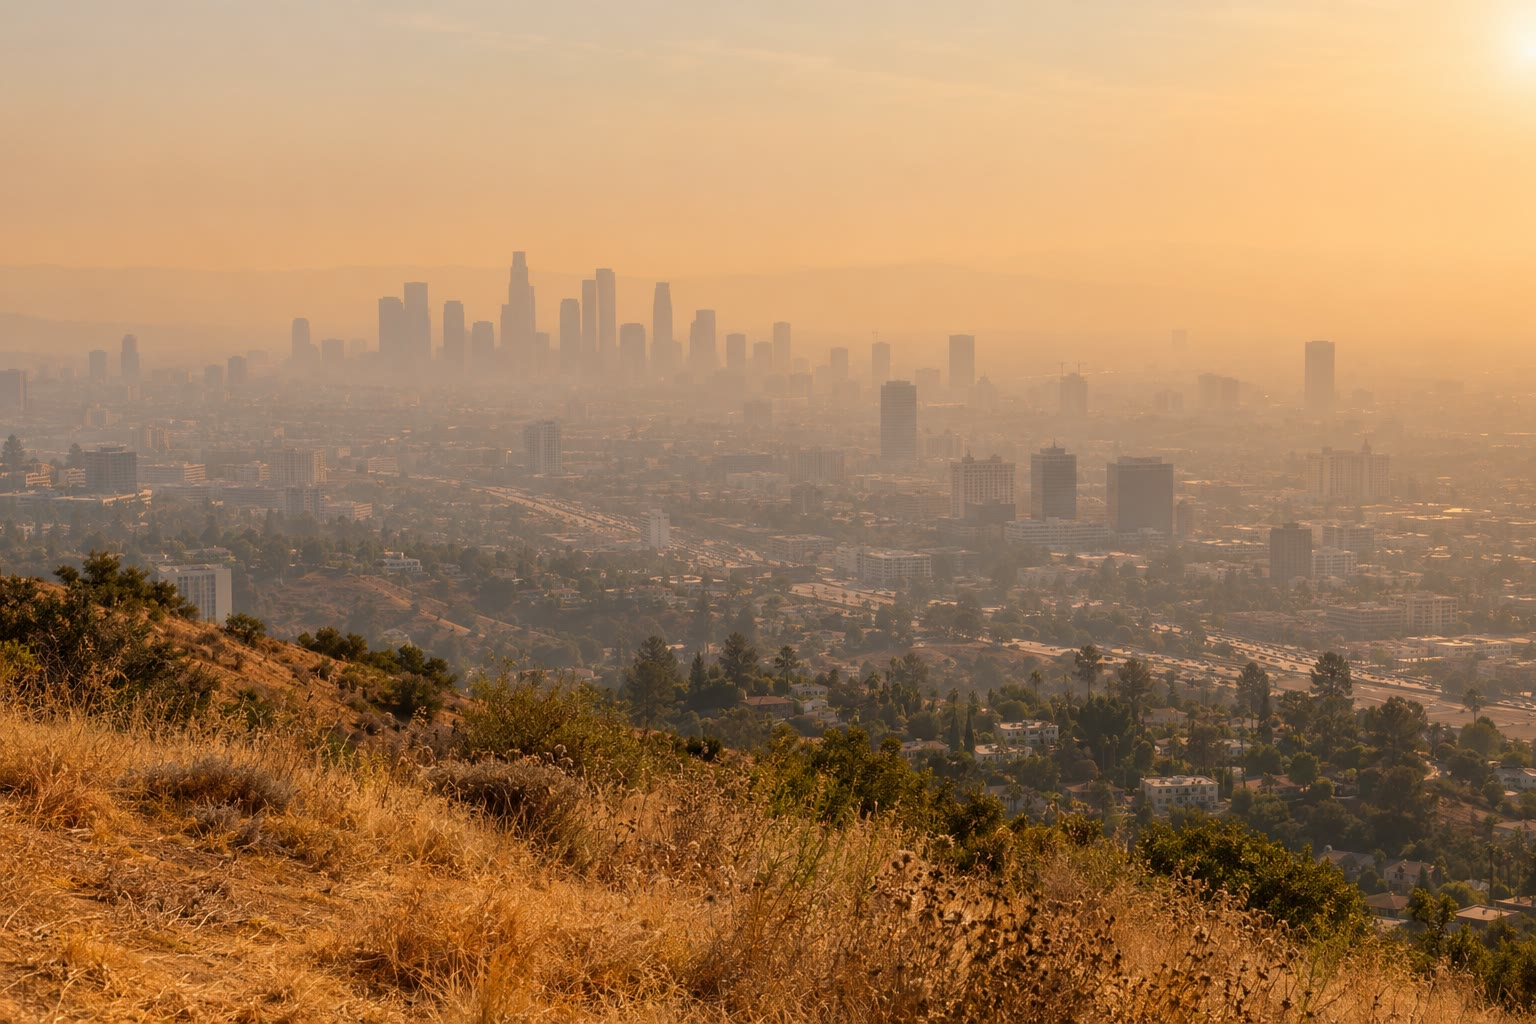
\includegraphics[width=0.6\linewidth]{images/book4/ai/b3-14-smog.jpg}

{\small مدينة تحت \omterm{def:b3:photochemistry:smog}{ضباب دخاني كيميائي ضوئي} في ظهيرة حارة. اللون البني يأتي
من \ce{NO2}؛ أما الأوزون، الذي يهيج الرئتين، فلا يُرى.}
\end{omfigure}

\begin{omfigure}
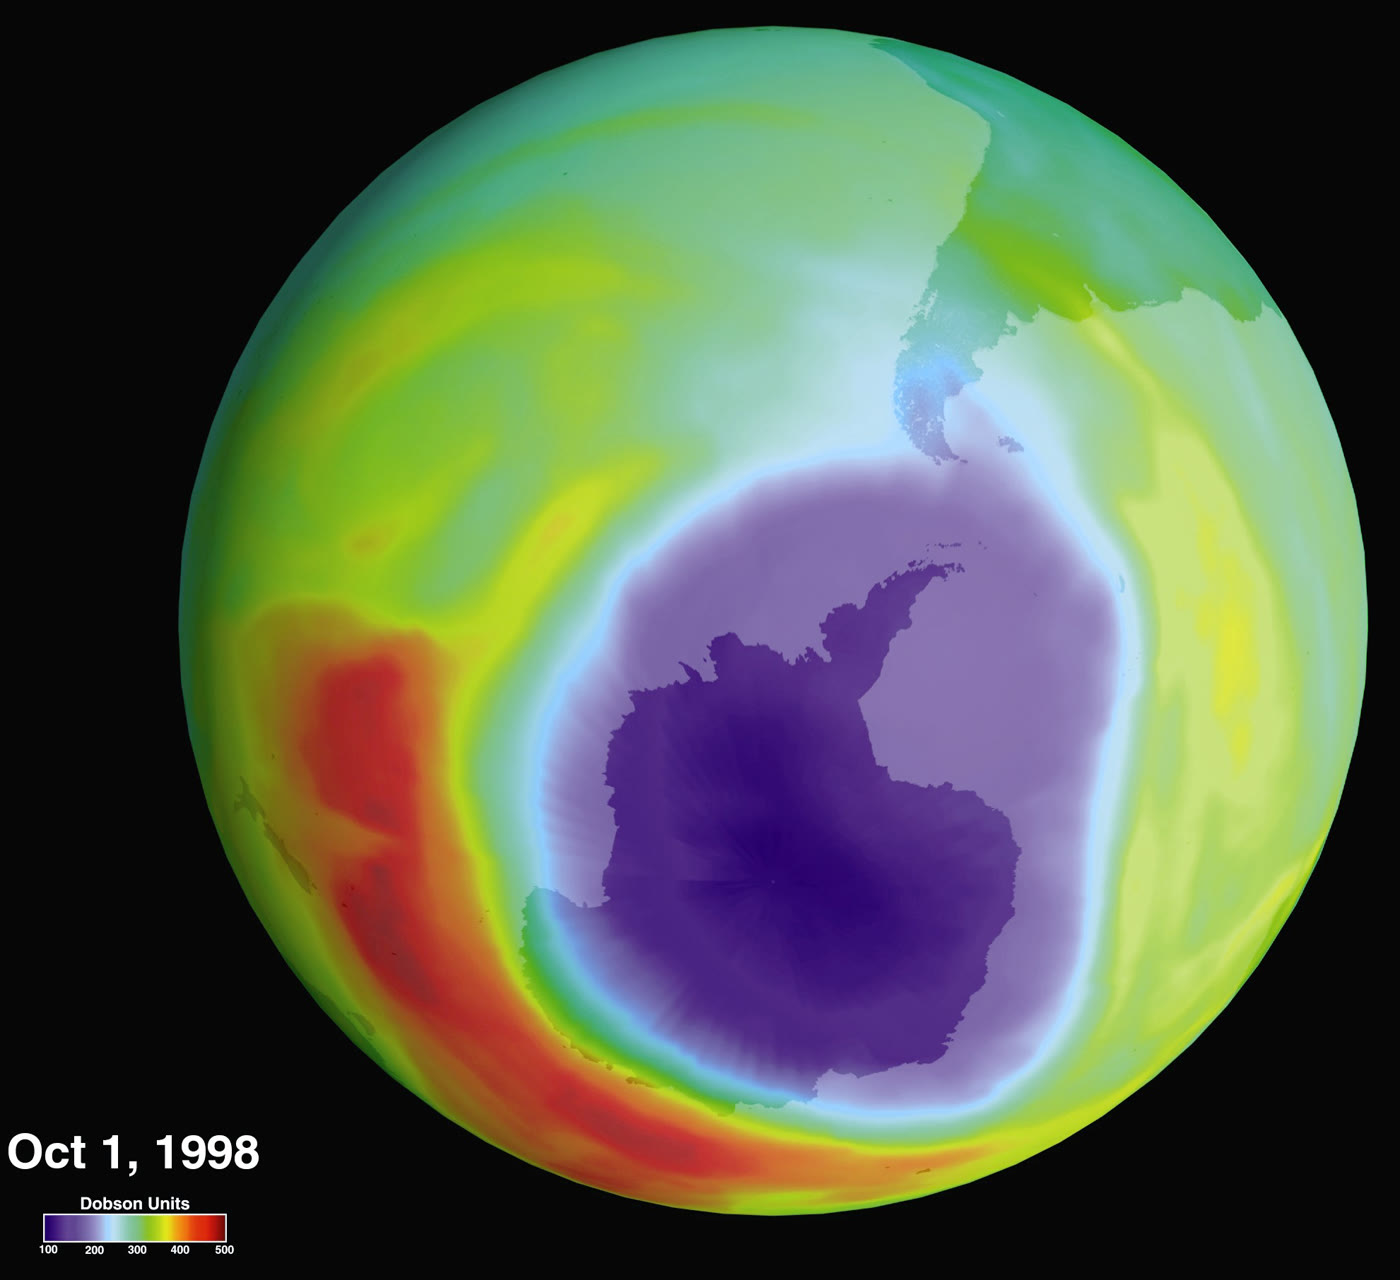
\includegraphics[width=0.5\linewidth]{images/book4/ozone-hole.jpg}

{\small عمود الأوزون فوق نصف الكرة الجنوبي في 1 أكتوبر 1998، من
قياسات الأقمار الصناعية: ينخفض ثقب الأوزون فوق القارة القطبية الجنوبية (البنفسجي) إلى نحو
100 وحدة دوبسون، مقابل نحو 300 في أماكن أخرى.}
\end{omfigure}

\begin{inthelab}[مفاعل ضوئي]
يتوسط وعاءَ التفاعل مصباحُ زئبق متوسط الضغط، مبرَّد في غلاف من الكوارتز؛
ويُزيل غلاف مرشح زجاجي الأطوال الموجية دون
نحو \qty{300}{nm}، التي قد تُتلف النواتج. ويُنزع الأكسجين من المحلول
بتيار من النيتروجين (فالأكسجين يُخمد الحالات الثلاثية) ويُحرَّك.
والمفاعل كله محجوب: فالمصباح يصدر أشعة فوق بنفسجية ضارة بالعينين
والجلد، ولا يُنظر إليه أبدًا، ولو لحظة.
\end{inthelab}

\begin{safety}{\ghs[0.8cm]{GHS08}\ghs[0.8cm]{GHS09}}
% ledger: ghs4:benzophenone
البنزوفينون، محسِّس شائع ومتفاعل الاختزال الضوئي:
يُشتبه في أنه يسبب السرطان، وقد يضر بالأعضاء بعد تعرض طويل،
وسام للأحياء المائية. يُوزن ويُتداول بالقفازات؛ وتذهب البقايا إلى
النفايات العضوية.
\end{safety}

\begin{history}[كيمياء المستقبل الضوئية، والثقب في السماء]
في سنة 1912 تساءل جاكومو تشاميتشيان، في بولونيا، هل يمكن للصناعة يومًا أن
تعمل بضوء الشمس، كما تفعل النباتات، بدل الفحم؛ وكان قد أمضى سنوات يعرّض
قوارير من المركبات العضوية للشمس على سطح مختبره. وفي سنة 1985،
أفاد ثلاثة علماء يعملون في محطة أبحاث في القارة القطبية الجنوبية بأن
عمود الأوزون الربيعي فوقها ينخفض بشدة منذ أواخر
السبعينيات.
وأدى ثقب الأوزون، الذي فسّرته في غضون سنوات قليلة كيمياء هذا الفصل،
إلى التخلص التدريجي من مركبات الكلوروفلوروكربون.
\end{history}

\section{تمارين}

\begin{exercise}[$\star$]\label{exo:b3:photochemistry:1}
مصباح يقدّم \qty{100}{mW} عند \qty{365}{nm}. كم فوتونًا في الثانية، وكم
أينشتاينًا في الثانية؟
\end{exercise}

\begin{exercise}[$\star$]\label{exo:b3:photochemistry:2}
في \qty{10.0}{min}، يحوّل محلول يمتص \qty{1.00e-7}{einstein.s^{-1}}
\qty{2.0e-5}{mol} من المتفاعل. احسب \omterm{def:b3:electronic-spectroscopy:quantum-yield}{المردود الكمي}.
\end{exercise}

\begin{exercise}[$\star$]\label{exo:b3:photochemistry:3}
للتفاعل الكيميائي الضوئي بين \ce{H2} و\ce{Cl2} مردودات كمية تبلغ $10^4$
وأكثر. ماذا يبيّن ذلك؟ اكتب خطوات الانتشار.
\end{exercise}

\begin{exercise}[$\star$]\label{exo:b3:photochemistry:4}
% ledger: janaf:O.dfH0, janaf:O3.dfH0
انطلاقًا من أنتالبيي التكوين عند 0 K للذرة O (\qty{246.79}{kJ/mol}) وللجزيء \ce{O3}
(\qty{145.35}{kJ/mol})، احسب أطول طول موجة يستطيع شطر \ce{O2} إلى ذرتين
وأطول طول موجة يستطيع شطر \ce{O3} إلى \ce{O2} وO.
\end{exercise}

\begin{exercise}[$\star\star$]\label{exo:b3:photochemistry:5}
لمبدّل ضوئي، عند \qty{365}{nm}، $\varepsilon_E = 22\,000$ و$\varepsilon_Z = 1500$ \unit{L.mol^{-1}.cm^{-1}}، مع
$\Phi_{E\to Z} = 0.11$ و$\Phi_{Z\to E} = 0.40$ (معطيات التمرين). احسب التركيب
المستقر ضوئيًا.
\end{exercise}

\begin{exercise}[$\star\star$]\label{exo:b3:photochemistry:6}
أعطِ نواتج \omterm{def:b3:photochemistry:norrish}{تفاعل نوريش من النوع الثاني} للهكسان-2-ون، وفسّر
لماذا يعطي البنتان-2-ون الإيثين بدل البروبين.
\end{exercise}

\begin{exercise}[$\star\star$]\label{exo:b3:photochemistry:7}
لمستقبل طاقة \omterm{def:b3:many-electron-atoms:singlet-triplet}{حالة ثلاثية} قدرها \qty{250}{kJ/mol}. ومن بين ثلاثة محسِّسات
مرشحة طاقات حالاتها الثلاثية 289 و253 و\qty{236}{kJ/mol} (معطيات
التمرين)، أيها ينقل بكفاءة؟ وقدّر ثابت توازن
النقل لكل منها عند \qty{298}{K}.
\end{exercise}

\begin{exercise}[$\star\star$]\label{exo:b3:photochemistry:8}
% ledger: kin:O+O2+M.k0, kin:O+O2+M.n
عند \qty{230}{K}، مع $[\mathrm M] = \qty{4.0e17}{cm^{-3}}$ و$[\ce{O2}] = 0.21[\mathrm M]$ و$j_3 = \qty{1.0e-3}{s^{-1}}$،
احسب $k_2$ والنسبة $[\ce{O}]/[\ce{O3}]$ في الحالة المستقرة.
\end{exercise}

\begin{exercise}[$\star\star$]\label{exo:b3:photochemistry:9}
% ledger: kin:Cl+O3.A, kin:Cl+O3.EaR, kin:Cl+CH4.A, kin:Cl+CH4.EaR
عند \qty{230}{K}، احسب ثابتي سرعة $\ce{Cl + O3}$ و$\ce{Cl + CH4}$، 
واحتمال أن تلتقي ذرة Cl بالجزيء \ce{O3} بدل \ce{CH4} حين $[\ce{O3}] = \qty{5.7e12}{cm^{-3}}$
و$[\ce{CH4}] = \qty{4.0e11}{cm^{-3}}$.
\end{exercise}

\begin{exercise}[$\star\star\star$]\label{exo:b3:photochemistry:10}
% ledger: kin:NO+O3.A, kin:NO+O3.EaR
عند الظهيرة في مدينة، $[\ce{NO2}]/[\ce{NO}] = 1.5$ و$j_{\ce{NO2}} = \qty{8.0e-3}{s^{-1}}$. احسب
الأوزون المستقر ضوئيًا عند \qty{298}{K} بالجزيئات في كل \unit{cm^3} وبالجزء من المليار (الهواء عند \qty{1}{bar}).
وماذا يحدث في الليل؟
\end{exercise}

\begin{exercise}[$\star\star\star$]\label{exo:b3:photochemistry:11}
محلول حجمه \qty{3.0}{mL} امتصاصيته 0.50 عند \qty{313}{nm} يتلقى \qty{50}{mW} من
الضوء عند طول الموجة هذا؛ وللتفاعل $\Phi = 0.25$. احسب السرعة الابتدائية بوحدة
\unit{mol.L^{-1}.s^{-1}}.
\end{exercise}

\begin{exercise}[$\star\star\star$]\label{exo:b3:photochemistry:12}
يكوّن مقياس أكتيني بالفيريأوكسالات، مردوده الكمي 1.25 عند \qty{365}{nm} (معطيات
التمرين) مع امتصاص كلي، \qty{3.0e-6}{mol} من Fe(II) في \qty{60}{s}.
احسب \omterm{def:b3:photochemistry:photon-flux}{تدفق الفوتونات}. ولماذا يجب أن يبقى التحويل صغيرًا؟
\end{exercise}

\section{مسألة: صنع طبقة الأوزون وهدمها}

\begin{problem}[{مسألة نهاية الأسبوع --- صنع طبقة الأوزون وهدمها: عتبات
الفوتونات، والحالة المستقرة لتشابمان بثوابت سرعة مقيَّمة، 
ودورة الكلور، والخزانات التي توقفها}]
\label{pb:b3:photochemistry:1}
% ledger: janaf:O.dfH0, janaf:O3.dfH0, kin:O+O2+M.k0, kin:O+O2+M.n, kin:O+O3.A, kin:O+O3.EaR, kin:Cl+O3.A, kin:Cl+O3.EaR, kin:O+ClO.A, kin:O+ClO.EaR, kin:Cl+CH4.A, kin:Cl+CH4.EaR, kin:ClO+NO2+M.k0, kin:ClO+NO2+M.n, kin:ClO+NO2+M.kinf, kin:ClO+NO2+M.Fc, oz:column.mean, oz:column.hole
نموذج للستراتوسفير قرب \qty{30}{km} (معطيات المسألة): $T = \qty{230}{K}$، $[\mathrm M] =
\qty{4.0e17}{cm^{-3}}$، $[\ce{O2}] = 0.21[\mathrm M]$، وثابتا سرعة \omterm{def:b3:photochemistry:photolysis}{التحلل الضوئي} $j_1 = \qty{1.0e-11}{s^{-1}}$ (\ce{O2})
و$j_3 = \qty{1.0e-3}{s^{-1}}$ (\ce{O3})، و$[\ce{CH4}] = \qty{4.0e11}{cm^{-3}}$، و$[\ce{NO2}] = \qty{1.0e9}{cm^{-3}}$. وثوابت السرعة
المقيَّمة (\unit{cm^3.s^{-1}}، أو \unit{cm^6.s^{-1}} من أجل $k_2$، مع عدّ التراكيز في كل \unit{cm^3}):
$k_2 = \num{6.0e-34}(T/300)^{-2.6}$؛ $k_4 = \num{8.0e-12}\eu^{-2060/T}$؛ Cl + \ce{O3}: $\num{2.8e-11}\eu^{-250/T}$؛
O + ClO: $\num{2.5e-11}\eu^{110/T}$؛ Cl + \ce{CH4}: $\num{6.6e-12}\eu^{-1240/T}$؛ ClO + \ce{NO2} + M: $\num{1.41e-13}$ في
هذه الظروف.

\medskip\noindent\textbf{الجزء الأول --- عتبات الفوتونات.}
\begin{enumerate}
  \item احسب $D_0(\ce{O2})$ من $\Delta_fH^\circ_0(\ce{O}) = \qty{246.79}{kJ/mol}$.
  \item استنتج أطول طول موجة يشطر \ce{O2}.
  \item احسب طاقة $\ce{O3 -> O2 + O}$ ($\Delta_fH^\circ_0(\ce{O3}) = \qty{145.35}{kJ/mol}$) وطول موجة
        العتبة الموافق لها.
  \item يستطيع الضوء المرئي إذن أن يشطر الأوزون؛ فلماذا يكون امتصاص الأوزون
        للأشعة فوق البنفسجية هو المهم للحياة؟
  \item لماذا لا يتحلل \ce{O2} ضوئيًا إلا في أعالي الغلاف الجوي؟
\end{enumerate}

\medskip\noindent\textbf{الجزء الثاني --- الحالة المستقرة لتشابمان.}
\begin{enumerate}[resume]
  \item اكتب خطوات تشابمان الأربع.
  \item احسب $k_2$ و$k_2[\mathrm M]$ عند \qty{230}{K}.
  \item احسب $k_4$.
  \item احسب $[\ce{O}]/[\ce{O3}]$.
  \item بيّن أن $[\ce{O3}] = [\ce{O2}]\sqrt{j_1k_2[\mathrm M]/(j_3k_4)}$.
  \item احسب $[\ce{O3}]$ ونسبة خلطه.
  \item احسب $[\ce{O}]$.
  \item الأوزون المرصود أقل من ذلك. لماذا؟
\end{enumerate}

\medskip\noindent\textbf{الجزء الثالث --- دورة الكلور.}
\begin{enumerate}[resume]
  \item اكتب الدورة وتفاعلها الصافي.
  \item احسب عمر ذرة Cl إزاء \ce{O3}.
  \item احسب عمر ClO إزاء O.
  \item استنتج النسبة المستقرة $[\ce{ClO}]/[\ce{Cl}]$.
  \item مع $[\ce{Cl}] + [\ce{ClO}] = \qty{1.0e7}{cm^{-3}}$، قارن سرعة فقد الأكسجين الفردي بالدورة
        بسرعة خطوة تشابمان $\ce{O + O3}$.
  \item أي خطوة تحدّ الدورة؟
\end{enumerate}

\medskip\noindent\textbf{الجزء الرابع --- الخزانات.}
\begin{enumerate}[resume]
  \item احسب احتمال أن تتفاعل ذرة Cl مع \ce{O3} بدل
        \ce{CH4}.
  \item احسب احتمال أن يتفاعل ClO مع O بدل \ce{NO2}.
  \item استنتج الاحتمال $p$ لاكتمال دورة.
  \item استنتج متوسط عدد الدورات قبل أن يُحتجز الكلور.
  \item فسّر كيف تطيل السحب الستراتوسفيرية القطبية السلسلة.
  \item اذكر النتيجة: عدد جزيئات الأوزون التي تُتلفها ذرة كلور
        واحدة، في هذا النموذج، قبل أن تُحتجز في خزان.
\end{enumerate}
\end{problem}
